 %!TEX root = report.tex

\subsection*{1.a}
For the assignment a launch file has to be created using Gmapping and teleoperation, which would finally save the map. The launch file is as follows:

\lstinputlisting[
	caption={The launch file to map the room.},
	label={lst:1:teleopMap}, 
	language=Python,
	float
]{./src/1/create_map.launch}

In order to get a map, the following commands have to be used in different terminals:

\begin{lstlisting}
	roslaunch navigation exercise1.launch
	roslaunch navigation create_map
\end{lstlisting}

\begin{itemize}
	\item \todo[inline]{De transforms gebeuren automagisch op basis van URDF, noem welke het zijn. zie GMapping wiki.}
\end{itemize}

\begin{figure}
	\centering
	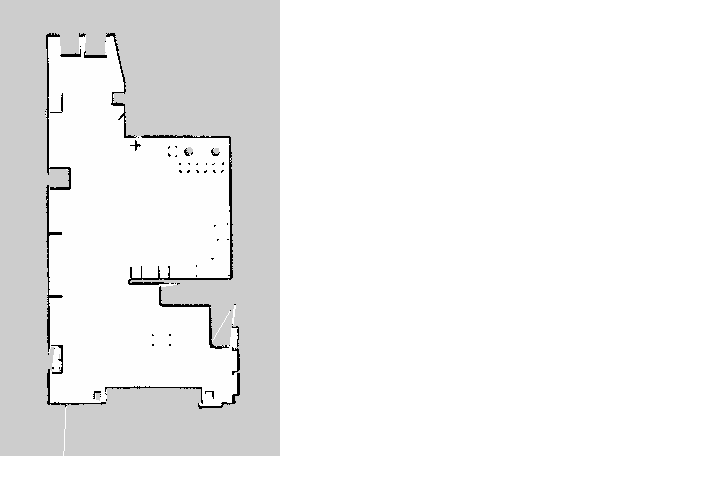
\includegraphics[width=\textwidth]{./img/map_teleop.png}
	\caption{The map that was made through mapping with teleop keyboard package.}
	\label{fig:1:map}
\end{figure}

\subsection*{1.b}

\todo[inline]{How do you run this?!}

For this assignment, the map from the first part had to be reused in Rviz, together with amcl. The following commands were necessary:

\begin{lstlisting}
	roslaunch navigation exercise1.launch
	roslaunch navigation amcl.launch
\end{lstlisting}

This gave a 2D map in Rviz, with an amcl representation of the robot in gazebo, as well as the 3D model in gazebo. In order to try and break the representations of the robot between Rviz and Gazebo, a lot of noise was introduced. Using this meant the rviz robot was at a different point than the gazebo robot after a while.

\lstinputlisting[
	caption={The launch file to map the room.},
	label={lst:2:teleopAmcl}, 
	language=Python,
	float
]{./src/1/amcl.launch}

\todo[inline]{add code to change location through python}
\todo[inline]{change speeds on robot}
\todo[inline]{show difference gazebo/rviz}